%%%%%%%%%%%%%%%%%%%%%%%%%%%%%%%%%%%%%%%%%%%%%%%%%%%%%%%%%%%%%%%%%%%%%
% PREAMBLE
%%%%%%%%%%%%%%%%%%%%%%%%%%%%%%%%%%%%%%%%%%%%%%%%%%%%%%%%%%%%%%%%%%%%%
%
% The following two commands will generate a PDF that follows all the requirements for submission
% and peer review.  Uncomment these commands to generate this output (and comment out the two lines below.)
%
% DOUBLE SPACE VERSION FOR SUBMISSION TO THE AMS
\documentclass[12pt]{article}
\usepackage{ametsoc}
%
% The following two commands will generate a single space, double column paper that closely
% matches an AMS journal page.  Uncomment these commands to generate this output (and comment
% out the two lines above. FOR AUTHOR USE ONLY. PAPERS SUBMITTED IN THIS FORMAT WILL BE RETURNED
% TO THE AUTHOR for submission with the correct formatting.
%
% TWO COLUMN JOURNAL PAGE LAYOUT FOR AUTHOR USE ONLY
%%%%\documentclass[10pt]{article}
%%%%\usepackage{ametsoc2col}
%
%%%%%%%%%%%%%%%%%%%%%%%%%%%%%%%%%%%%%%%%%%%%%%%%%%%%%%%%%%%%%%%%%%%%%
% ABSTRACT
%
% Enter your Abstract here
%%%%%%%%%%%%%%%%%%%%%%%%%%%%%%%%%%%%%%%%%%%%%%%%%%%%%%%%%%%%%%%%%%%%%
\newcommand{\myabstract}{
Direct measurements of entrainment and detrainment rates from LES model 
cloud fields produce values twice as large as those produced from bulk 
conserved tracer budget calculations.  This difference can be explained by 
three effects: the presence of a shell of moist air around the clouds, Reynolds 
correlations between entrainment rates and tracer values, and numerical errors 
in the calculation methods.  Correlations between the vertical momentum and the
entrainment rate create strong vertical momentum Reynolds fluxes, making the 
assumption that clouds entrain fluid with zero vertical momentum incorrect.  
Variability in the properties of the moist cloud shell has strong impacts on 
entrainment values inferred from bulk tracer calculations.  These results 
indicate the dynamics of the cloud shell should be included in 
parameterizations of cumulus clouds used in general circulation models.
}
%
\begin{document}
%
%%%%%%%%%%%%%%%%%%%%%%%%%%%%%%%%%%%%%%%%%%%%%%%%%%%%%%%%%%%%%%%%%%%%%
% TITLE
%
% Enter your TITLE here
%%%%%%%%%%%%%%%%%%%%%%%%%%%%%%%%%%%%%%%%%%%%%%%%%%%%%%%%%%%%%%%%%%%%%
\title{\textbf{\large{The influence of the cloud shell on bulk tracer 
measurements of LES cloud entrainment}}}
%
% Author names, with corresponding author information. 
% [Update and move the \thanks{...} block as appropriate.]
%
\author{\textsc{Jordan T Dawe}
				\thanks{\textit{Corresponding author address:} 
				Jordan T Dawe, Department of Earth and Ocean Sciences, 
                                University of British Columbia, 6339 Stores Road,
                                Vancouver, BC, V6T 1Z4, Canada.
				\newline{E-mail: jdawe@eos.ubc.ca}}\quad\textsc{and Philip H Austin}\\
\textit{\footnotesize{Department of Earth and Ocean Sciences, University of 
                      British Columbia, Vancouver, BC, Canada.}}
}
%
% Formatting done here...Authors should skip over this.  See above for abstract.
\ifthenelse{\boolean{dc}}
{
\twocolumn[
\begin{@twocolumnfalse}
\amstitle

% Start Abstract (Enter your Abstract above.  Do not enter any text here)
\begin{center}
\begin{minipage}{13.0cm}
\begin{abstract}
	\myabstract
	\newline
	\begin{center}
		\rule{38mm}{0.2mm}
	\end{center}
\end{abstract}
\end{minipage}
\end{center}
\end{@twocolumnfalse}
]
}
{
\amstitle
\begin{abstract}
\myabstract
\end{abstract}
}
%%%%%%%%%%%%%%%%%%%%%%%%%%%%%%%%%%%%%%%%%%%%%%%%%%%%%%%%%%%%%%%%%%%%%
% MAIN BODY OF PAPER
%%%%%%%%%%%%%%%%%%%%%%%%%%%%%%%%%%%%%%%%%%%%%%%%%%%%%%%%%%%%%%%%%%%%%
\section{Introduction}

The rate at which air is entrained into and detrained from clouds affects cloud 
properties, cloud top height, and vertical transports of heat and moisture.  
Proper simulation of these subgrid-scale effects in General Circulation Models 
(GCM) depends on the accurate parameterization of entrainment and detrainment 
\citep{Bechtold2008,Rougier2009,De_Rooy2010}.

Large Eddy Simulation (LES) is a primary tool used to study these dynamics.  
LES entrainment and detrainment rates are typically calculated using budgets of 
bulk conserved tracer variables to inferring the amount of fluid exchange 
between the clouds and the surrounding air.  These rates are then used in 
simple entraining plume parameterizations to evaluate sub-grid scale cloud 
transports.  \cite{Siebesma1995} derive the following equations for 
entrainment and detrainment from a cloud core plume, where cloud core is 
defined as regions having condensed liquid water, positive buoyancy, and upward 
vertical velocity:
\begin{equation}
  \label{eq:siebesma_entrainment}
    E_{\phi}(\phi_c - \phi_e) = - M_c \frac{\partial \phi_c}{\partial z}
        - \frac{\partial \rho a \overline{w' \phi'}^c}{\partial z}
        - \rho a \frac{\partial \phi_c}{\partial t}
        + a \rho \left(\frac{\partial \bar{\phi}}{\partial t}\right)_{forcing}
\end{equation}
and
\begin{equation}
  \label{eq:siebesma_detrainment}
    D_{\phi}(\phi_c - \phi_e) = - M_c \frac{\partial \phi_e}{\partial z}
        + \frac{\partial \rho (1 - a) \overline{w' \phi'}^e}{\partial z}
        + \rho (1-a) \frac{\partial \phi_e}{\partial t}
     - \rho (1-a) \left(\frac{\partial \bar{\phi}}{\partial t}\right)_{forcing}
\end{equation}
Here $\phi$ represents any conserved bulk tracer, such as the total specific 
humidity $q_t$ (kg water kg$^{-1}$ moist air) or the liquid-water moist static 
energy $h$ (J kg$^{-1}$), $a$ is the fractional cloud core area, $\rho$ is the 
density of the air in kg m$^{-3}$, $M_c$ is vertical cloud core mass flux 
(kg m$^{-2}$ s$^{-1}$), $w$ is vertical velocity (m s$^{-1}$), $e$ and $c$ sub- 
and super-scripts denote horizontally averaged values conditionally sampled in 
the cloud environment and core, $forcing$ refers to tracer sources and sinks,
such as radiation or subsidence, not included in the other terms, primed values 
represent anomalies relative to the horizontal mean, overbars represent 
horizontal averaging, and $E_{\phi}(z)$ and $D_{\phi}(z)$ are the total bulk 
tracer entrainment into and detrainment out of the cloud core in 
kg s$^{-1}$ m$^{-3}$.  

Alternatively, entrainment and detrainment can be calculated directly from the 
LES velocity and tracer fields.  \cite{Romps2010} recently presented a 
technique to measure entrainment and detrainment in this manner.  His equation (2) is:
\begin{equation}
  \label{eq:romps_e_minus_d}
  e - d = \frac{\partial}{\partial t}(\mathcal{A}\rho) 
        + \nabla \cdot (\rho \mathbf{u} \mathcal{A}) 
\end{equation}
Here $e(x,y,z)$ and $d(x,y,z)$ are the local entrainment and detrainment through 
the cloud core surface in kg s$^{-1}$ m$^{-3}$, $\mathbf{u}$ is the velocity of 
the air in m s$^{-1}$, and $\mathcal{A}$ is the ``activity" of the fluid, where 
$\mathcal{A}$ is one at ``active" cloud core points and zero otherwise.  The 
values of $e - d$ are averaged over the time that a grid cell experiences mass 
fluxes between an active and an inactive point, then positive $e-d$ values 
are considered to be purely $e$, and negative values, $d$.  Summing these point 
measurements horizontally gives $E_d(z)$ and $D_d(z)$, the total directly 
calculated cloud core entrainment and detrainment in kg s$^{-1}$ m$^{-3}$.

Romps found that direct measurement of the fluxes produced values roughly twice 
as large as tracer budget calculations.  Romps attributed this difference to 
the bulk tracer calculation assumption that fluid exchanged between clouds 
and environment has the mean properties of the cloud or environment, 
respectively.  The unlikeliness of this assumption is suggested by recent 
studies of the dense, descending shell of moist air that forms around 
trade-wind cumulus clouds \citep{Heus2008, Wang2010}.  Since fluid exchanges 
between clouds and environment must pass through this shell, it is likely that 
it plays an important role in entrainment and detrainment dynamics.

Reconciling the direct flux and bulk tracer calculations is important if direct 
flux calculations are to inform GCM parameterizations.  Here we examine the 
sources of the discrepancy between the methods.  We show the discrepancy is 
explained by three effects: the presence of the moist shell, correlations 
between the entrainment rates and the tracer values which cause Reynolds 
fluxes, and numerical errors in the calculation methods.  We derive a 
correction to convert between ``tracer" and ``direct" entrainment fluxes, and 
then use this correction to evaluate the impact of variability in the moist 
shell on bulk tracer entrainment and detrainment rates.

%===================================================

\section{Model description}

All LES calculations in this paper were made using the System for Atmospheric 
Modeling \citep[SAM;][]{Khairoutdinov2003}.  Two model runs were performed, 
configured as standard Global Energy and Water Cycle Experiment (GEWEX) 
Cloud System Studies \citep[GCSS;][]{Randall2003} experiments: a Barbados 
Oceanographic and Meteorological Experiment \citep[BOMEX;][]{Siebesma2003} run,
and an Atmospheric Radiation Measurement Study \citep[ARM;][]{Brown2002} run. 
The BOMEX run was performed on a 6.4 km x 6.4 km horizontal x 3.2 km vertical 
domain with 25 meter grid resolution in all directions for 6 hours, and the 
first three hours of simulation were discarded. The ARM run was performed on a 
7.68 km x 7.68 km x 4.5 km domain with 30 meter grid resolution.

We have implemented the entrainment calculation scheme of \cite{Romps2010} in 
SAM, allowing us to calculate cloud core entrainment and detrainment directly 
from model mass fluxes.  \citet[eq. 4]{Romps2010} also presents a method for 
calculating tracer entrainment rates in the same framework as 
(\ref{eq:romps_e_minus_d}), but neglects forcing and diffusion terms.  These 
are significant for tracer quantities like vertical momentum, so we retain 
these terms in Romps's tracer equation:
\begin{equation}
  \label{eq:romps_ephi_minus_dphi}
  e\phi - d\phi = \frac{\partial}{\partial t}(\phi \mathcal{A} \rho) 
                + \nabla \cdot (\phi \rho \mathbf{u} \mathcal{A})
                - \mathcal{A}S_\phi
\end{equation}
where $S_\phi$ is any non-advective source term for $\phi$, in units of 
$[\phi]$ s$^{-1}$.  This equation is then averaged in the same way as equation 
(\ref{eq:romps_e_minus_d}), but since $\phi$ can be negative, negative 
entrainment fluxes are now possible.  If the average value of $\phi$ over the 
period of flux averaging is positive, then positive $e\phi-d\phi$ values are 
considered to be purely $(e\phi)(x,y,z)$, and negative values, 
$(d\phi)(x,y,z)$.  However, if $\phi$ is negative then positive $e\phi-d\phi$ 
values are considered to be purely $(d\phi)(x,y,z)$, and negative values, 
$(e\phi)(x,y,z)$.  Horizontal summation then gives $(E\phi)_d(z)$ and 
$(D\phi)_d(z)$, the total directly calculated tracer entrainment and 
detrainment for the cloud ensemble in $[\phi]$ kg s$^{-1}$ m$^{-3}$.

%===================================================

\section{The Cloud Shell}

To quantify the effect of the moist cloud shell on entrainment and detrainment
we define average or effective tracer values $\phi_E = (E\phi)_d / E_d$ and 
$\phi_D = (D\phi)_d / D_d$.  Examination of these values from the BOMEX 
simulation using total specfic humidity shows significant differences between 
$q_E$ and the environmental $q_t$ and between $q_D$ and the core $q_t$ (Figure 
\ref{fig:Reynolds_correction}a), confirming that $q_E$ and $q_D$ differ from
the mean environment and core values.

Calculated $q_D$ agrees well with the mean ``cloud core edge" (cloud core model 
grid cells that are nearest-neighbor adjacent to non-core cells) $q_t$ values.  
$q_E$, however, is moister than the mean ``cloud core shell" (non-core model 
grid cells that are nearest-neighbor adjacent to core cells) values.  This 
suggests that non-trivial Reynolds fluxes exist between $q_E$ and $e$: more 
entrainment occurs when $q_t$ is larger than the mean $q_t$ of the shell air, 
and less when $q_t$ is smaller.

%-------------------------------------------------------------------------

\subsection{$E$ and $D$ correction}
  
Here we derive a correction to equations (\ref{eq:siebesma_entrainment}) and 
(\ref{eq:siebesma_detrainment}) to account for the presence of the moist cloud 
shell and dry cloud edge, allowing us to convert between ($E_d, D_d$) and 
($E_\phi, D_\phi$).  We start our derivation by modifying equation (5.1) from
\cite{Siebesma1995}:
\begin{eqnarray}
  \label{eq:entrainment_derivation_1}
    \rho \frac{\partial a \phi_c}{\partial t} 
    = - \frac{\partial M_c \phi_c}{\partial z} 
    + E_d \phi_E - D_d \phi_D
    - \frac{\partial \rho a \overline{w' \phi'}^c}{\partial z} 
    + a \rho \left(\frac{\partial \bar{\phi}}{\partial t}\right)_{forcing}
\end{eqnarray}
\begin{eqnarray}
  \label{eq:detrainment_derivation_1}
    \rho \frac{\partial (1 - a) \phi_e}{\partial t}
    = \frac{\partial M_c \phi_e}{\partial z} 
    - E_d \phi_E + D_d \phi_D
    - \frac{\partial \rho (1 - a) \overline{w' \phi'}^e}{\partial z} 
    + \rho (1 - a) \left(\frac{\partial \bar{\phi}}{\partial t}\right)_{forcing}.
\end{eqnarray}
Here we have replaced $\phi_e$ in the entrainment term with $\phi_E$ and 
$\phi_c$ in the detrainment term with $\phi_D$, where $\phi_E$ and $\phi_D$ are 
the bulk tracer value of the air being entrained and detrained, respectively.

Next we substitute into (\ref{eq:entrainment_derivation_1}) and
(\ref{eq:detrainment_derivation_1}) the continuity equation for a cloud plume,
\begin{equation}
   \label{eq:continuity}
   \rho \frac{\partial a}{\partial t} 
   + \frac{\partial M_c}{\partial z} = E_d - D_d,
\end{equation}
allowing us to write
\begin{eqnarray}
  \label{eq:entrainment_derivation_2}
    E_d (\phi_c - \phi_E) - D_d (\phi_c - \phi_D)
    = M_c \frac{\partial \phi_c}{\partial z}
    + \frac{\partial \rho a \overline{w' \phi'}^c}{\partial z} 
    + \rho a \frac{\partial \phi_c}{\partial t}
    - a \rho \left(\frac{\partial \bar{\phi}}{\partial t}\right)_{forcing}
\end{eqnarray}
\begin{eqnarray}
  \label{eq:detrainment_derivation_2}
    D_d (\phi_D - \phi_e) - E_d (\phi_E - \phi_e)
    = - M_c \frac{\partial \phi_e}{\partial z}
    + \frac{\partial \rho (1 - a) \overline{w' \phi'}^e}{\partial z} 
    + \rho (1 - a) \frac{\partial \phi_e}{\partial t}
    - \rho (1 - a) \left(\frac{\partial \bar{\phi}}{\partial t}\right)_{forcing}.
\end{eqnarray}

Finally, we substitute in equations (\ref{eq:siebesma_entrainment}) and 
(\ref{eq:siebesma_detrainment}) for the bulk tracer tendency terms and 
rearrange to get
\begin{equation}
  \label{eq:corrected_entrainment}
    E_{\phi} = E_d - E_d\frac{\phi_E - \phi_e}{\phi_{c} - \phi_{e}}
             - D_d\frac{\phi_c - \phi_D}{\phi_{c} - \phi_{e}}
\end{equation}
\begin{equation}
  \label{eq:corrected_detrainment}
    D_{\phi} = D_d - D_d\frac{\phi_c - \phi_D}{\phi_{c} - \phi_{e}}
             - E_d\frac{\phi_E - \phi_e}{\phi_{c} - \phi_{e}}.
\end{equation}
Note that under this correction $E_d-D_d = E_{\phi}-D_{\phi}$, preserving 
mass continuity.

Comparison of $E_{q_t}$ and $D_{q_t}$ ($E_{\phi}$ and $D_{\phi}$ inferred using 
specific humidity $q_t$ as the bulk tracer) with $E_d$ and $D_d$ calculated by 
the method of \cite{Romps2010} shows the directly calculated values are 
significantly larger than the bulk tracer values (Figure 
\ref{fig:Reynolds_correction}, b and c).  Correcting $E_d$ and $D_d$ using the 
mean $q_t$ of the cloud core edge and shell in place of $q_E$ and $q_D$ in 
equations (\ref{eq:corrected_entrainment}) and (\ref{eq:corrected_detrainment})
improves the agreement with the bulk tracer calculations.  Relative to the bulk 
tracer calculation, the corrected $E_{q_t}$ values are still too large near 
cloud base.  However, the correction does duplicate the negative $D_{q_t}$ 
values near cloud base that are typically produced by bulk tracer calculations.

Including the effect of Reynolds correlations by using $q_E = (E q_t)_d/E_d$ 
and $q_D = (D q_t)_d/D_d$ decreases the corrected $E_d$ and $D_d$ values even 
further (Figure \ref{fig:Reynolds_correction}, b and c).  This reduces the 
correction agreement with the bulk tracer calculation over most of the cloud 
layer, but also reduces the large entrainment values near cloud base, improving 
the overall shape of the fluxes.  Still, the entrainment values corrected by 
$q_E$ and $q_D$ are about half the magnitude of the Siebesma bulk tracer 
values.

This overcorrection is the result of numerical errors due to the discrete 
grid on which the LES fluxes are calculated.  To show this, we use alternate 
equations for the calculation of bulk tracer entrainment and detrainment, 
derived by \cite{Romps2010}:
\begin{equation}
  \label{eq:romps_bulk_entrainment}
    E_{\phi}(\phi_c - \phi_e) = \phi_c(E_d-D_d) - ((E\phi)_d - (D\phi)_d)
\end{equation}
\begin{equation}
  \label{eq:romps_bulk_detrainment}
    D_{\phi}(\phi_c - \phi_e) = \phi_e(E_d-D_d) - ((E\phi)_d - (D\phi)_d)
\end{equation}
Note that by substituting $(E\phi)_d = E_d \phi_E$ and $(D\phi)_d = D_d \phi_D$ 
into (\ref{eq:romps_bulk_entrainment}) and (\ref{eq:romps_bulk_detrainment}),
we can quickly recover (\ref{eq:corrected_entrainment}) and 
(\ref{eq:corrected_detrainment}).  Because of this, the Romps bulk tracer 
formulation agrees exactly with the result of the $q_E$ and $q_D$ correction,
producing smaller $E_{q_t}$ and $D_{q_t}$ values than the Siebesma bulk tracer 
calculation.  

Siebesma's bulk tracer calculation estimates vertical tracer fluxes from the 
mean profiles of tracer quantities, while Romps' calculation finds the flux for 
each grid cell directly from the numerical model's advection code.  Romps' 
calculation is therefore much more consistent with the model formulation than 
Siebesma's.  Conversely, Romps' calculation requires finding the difference of 
two large quantities ($\phi_c(E_d-D_d)$ and $(E\phi)_d - (D\phi)_d$), with all 
the numerical problems that implies.  Both these calculation methods therefore 
are subject to numerical errors that reduce their accuracy.  

%------------------------------------------------------------------------------

\subsection{$h$, $w$, and Reynolds correlations}

Since Reynolds correlations between $e$ and $q_t$ appear to have an important 
effect on the measured moisture fluxes between cloud and environment, we now 
examine energy fluxes, represented in SAM by the liquid water moist static 
energy $h$ (units of J kg$^{-1}$) and the vertical momentum, represented in SAM 
by the vertical velocity $w$ (units of m s$^{-1}$).

Liquid water moist static energy shows a similar distribution of core, edge, 
shell, environment, $h_E$ and $h_D$ properties when compared to $q_t$, 
indicating a tight coupling between these variables in the cloud dynamics 
(Figure \ref{fig:profile_plots}a).  Near cloud base, edge, shell, $h_E$ and 
$h_D$ all converge on the core value, spreading out in the cloud layer and 
becoming relatively more core-like in the inversion.  $h_D$ is identical to the 
edge properties, while $h_D$ is smaller than $h$ in the shell, indicating the 
influence of Reynolds flux correlations between $e$ and $h$.

We can quantify the effect of these Reynolds fluxes by looking at 
$A = (h_E - h_e)/(h_c - h_e)$ and $B = (h_c - h_D)/(h_c - h_e)$, the correction 
factors in equations (\ref{eq:corrected_entrainment}) and 
(\ref{eq:corrected_detrainment}).  Using the edge and shell values of $h$ for 
$h_E$ and $h_D$ shows $A$ to have a much larger effect than $B$, due to the 
larger difference between the shell and the environment than between the edge 
and the core.  $E_d$ is reduced by 0.2 by the $A$ correction, while 0.45 of
$D_d$ is removed by $B$.  If instead we use $h_E = (E h)_d/E_d$ and 
$h_D = (D h)_d/D_d$ in equations (\ref{eq:corrected_entrainment}) and 
(\ref{eq:corrected_detrainment}), $A$ is unchanged but $B$ increases to 0.6.  
Calculations for $q_t$ values show nearly identical results (not shown).

Vertical velocity shows very different relative profiles compared to
$q_t$ and $h$.  There is a much wider spread in the $w$ values,
with the shell having nearly zero vertical velocity and the edge being
halfway between the core and the environment.  $w_D$ is again similar
to the value of $w$ in the edge, but $w_E$ is much larger than $w$ in
the shell, and in fact is roughly the same value as $w_D$ over most of
the cloud layer.  This large positive value for $w_E$ is clearly inconsistent
with the assumption made in many entraining plume models that 
fluid entrained into the cloud core plume has negligible vertical momentum
\citep{Simpson1969,Gregory2001,Siebesma2003}

These differences indicate that Reynolds correlations are much more important 
to the $w$ fluxes than the $q_t$ or $h$ fluxes.  Indeed, using the value 
of $w$ in the shell to calculate term $A$ results in a value of only about 0.2, 
while using $w_E$ increased $A$ to 0.45.  Term $B$ shows much less sensitivity 
to the Reynolds fluxes, but is still reduced by about 0.1 by substituting $w_D$ 
for the edge value of $w$.

%-------------------------------------------------------------------------

\subsection{Instantaneous Fields}

The source of these Reynolds fluxes, and the reason they affect $w$ more than 
$q_t$ or $h$, can be seen by comparing instantaneous snapshots of the model 
values $e$, $e_{q_t}$, and $e_w$.  Since \cite{Romps2010} method of calculating 
$e$ and $d$ requires long time averages over the period that the cloud surface
is adjacent to a grid cell, it is unfortunately unsuitable for calculating 
instantaneous fields.  Instead, we use an alternative method we have devised 
that substitutes spatial interpolation for time averaging \citep{Dawe2011}.  
This alternative method results in slightly smaller values of $e$ and $d$ than 
are produced by Romps' method, but the two calculations show good agreement in 
variability. $eq_t$ and $ew$ are calculated simply by multiplying the value 
of $e$ by the values of $q_t$ and $w$, respectively.

Examination of these fields shows that, while $e$ and $eq_t$ have a very 
similar spatial pattern, $ew$ is concentrated in regions where strong updrafts 
enter the cloud core (Figure \ref{fig:w_entrainment_example}).  The reason for 
this can been seen by examining the buoyancy, condensed liquid water,
and vertical velocity fields that define the cloud core.  Of these three
fields, buoyancy is the strongest constraint on the core.  However, regions 
exist far above cloud base where air has become negatively buoyant but 
maintains upward velocity and elevated moisture.  As this air continues to 
rise more condensation occurs, which heats the updraft, makes it positively 
buoyant, and thus entrains it into the core.  In this way, entrainment is 
positively correlated with both $q_t$ and $w$.  This process occurs fairly 
often in our model cloud field, as evidenced both by our manual examination of 
the output fields, and the size of the Reynolds flux terms in the mean 
profiles.

%-------------------------------------------------------------------------

\subsection{Shell Variability}

Finally we ask whether variability of the shell and edge properties has an 
impact on the measured variability in the bulk tracer calculations of $E$ and 
$D$.  To do this we turn to the ARM run, and simply look at the variability in 
$A = (q_E - {q_t}_e)/({q_t}_c - {q_t}_e)$ and 
$B = ({q_t}_c - q_D)/({q_t}_c - {q_t}_e)$.  These quantities indeed show 
strong variability over the ARM diurnal cycle (Figure 
\ref{fig:shell_variability}).  Near cloud base and within the inversion, $A$ 
is nearly one while $B$ is nearly zero.  As the clouds mix into the inversion 
over the course of the day, the values evolve until at mid-cloud layer, $A$ 
has values near 0.6 and $B$ near 0.2.  Performing this calculation with a fixed 
value of $({q_t}_c - {q_t}_e)$, to remove changes due to movement of the mean 
environment and core profiles, shows similar results.  The shell is clearly an 
active player in the entrainment and detrainment fluxes.

%==============================================================================

\section{Discussion and Conclusion}

We have explained the differences between entrainment and detrainment values 
calculated via bulk tracer budgets and direct flux calculations by taking into 
account the properties of the cloud shell, the effect of Reynolds fluxes, and 
differences in the numerical methods used by the two calculations.  This 
suggests that the presence of the moist cloud shell has a significant role in 
mediating fluxes between the clouds and the environment and may be an important 
factor in improving parameterizations of shallow convection.

Significant Reynolds fluxes are apparent in tracer and vertical momentum 
entrainment.  These fluxes are the result of vertical advection of moist but 
negatively buoyant air so that condensation causes latent heating, making the 
air buoyant and entraining it into the core.  However, this process is not 
unique to the definition of cloud core.  Similar correlations appear when we 
perform these calculations for regions of condensed liquid water, as vertical 
advection can drive cloud condensation and thus cause entrainment.

Whether one considers the bulk tracer or directly calculated flux values to be 
``correct" will depend on the purpose for which they are used.  The bulk tracer 
values are well suited to calculating fluxes in GCM sub-grid scale 
parameterizations, which only have access to large-scale values.  The influence 
of variability in the cloud shell would then simply be incorporated into the 
parameterization of the bulk tracer entrainment and detrainment values.  On the 
other hand, direct fluxes may be needed for calculating fluxes of aerosols whose 
chemical properties are altered by reactions in the presence of liquid water 
\citep{Hoppel1994}.

\begin{acknowledgment} 
Support for this work was provided by the Canadian Foundation for Climate and 
Atmospheric Science through the Cloud Aerosol Feedback and Climate network.
We thank Marat Khairoutdinov for making SAM available to the cloud modeling 
community.  All figures were generated using the matplotlib library in the 
Python programming language.
\end{acknowledgment}

% Use appendix}[A], {appendix}[B], etc. etc. in place of appendix if you have multiple appendixes.
\ifthenelse{\boolean{dc}}
{}
{\clearpage}

% Create a bibliography directory and place your .bib file there.
\ifthenelse{\boolean{dc}}
{}
{\clearpage}
\bibliographystyle{ametsoc}
\bibliography{./bibliography/shell_correction}

%%%%%%%%%%%%%%%%%%%%%%%%%%%%%%%%%%%%%%%%%%%%%%%%%%%%%%%%%%%%%%%%%%%%%
% FIGURES
%%%%%%%%%%%%%%%%%%%%%%%%%%%%%%%%%%%%%%%%%%%%%%%%%%%%%%%%%%%%%%%%%%%%%

\begin{figure}[t]
  \noindent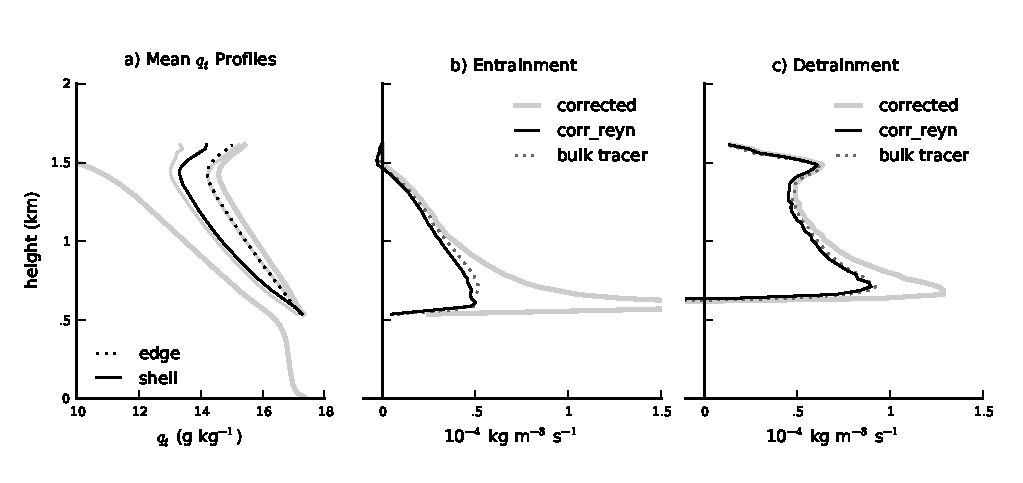
\includegraphics[width=39pc,angle=0]{./figures/reynolds_correction}\\
  \caption{Result of correcting direct entrainment values for the presence of 
  the moist cloud shell.  a) Mean profiles of the effective total specific 
  humidity values being entrained ($q_E$, black line), and detrained ($q_D$ dotted 
  line), overlaid on the total specific humidity in the cloud core (thick dark 
  grey line), cloud core edge (thin dark grey line), cloud core shell (thin 
  grey line), and cloud core environment (thick grey line).  These $q_t$ values 
  are used to correct values of b) entrainment and c) detrainment; shown are the 
  direct flux calculation of \cite{Romps2010} (thick grey line), the bulk 
  tracer budget calculation of \cite{Siebesma1995} (dotted line), the direct 
  flux calculation corrected by the mean core shell and edge values (``shell/edge corrected'', thin grey 
  line), and the direct flux calculation corrected by the $q_E$ and $q_D$ 
  values (``$q_E/q_D$ corrected'', black line).}
  \label{fig:Reynolds_correction}
\end{figure}

\begin{figure}[t]
  \noindent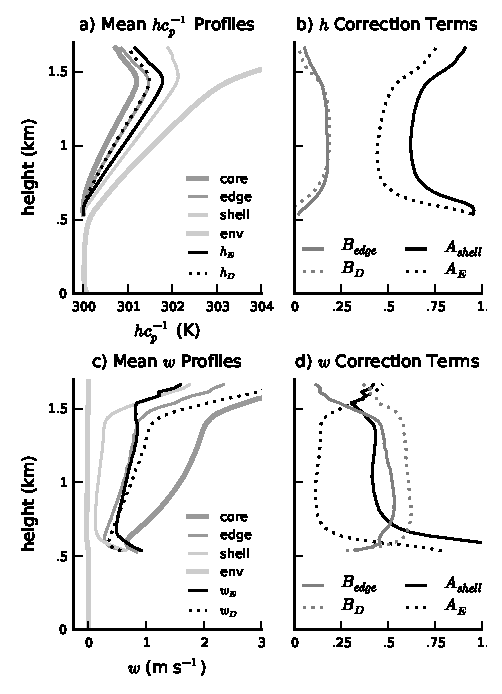
\includegraphics[width=19pc]{./figures/profile_plots}
  \caption{Mean profiles of a) liquid-water moist static energy values for 
  entraining (black line) and detraining (dotted line) air, overlaid on the 
  mean core, edge, shell, and environment profiles (grey lines), and b) the 
  resulting $A_{shell} = (h_{shell} - h_e)/(h_c - h_e)$, 
  $A_E = (h_E - h_e)/(h_c - h_e)$,  
  $B_{edge} = (h_c - h_{edge})/(h_c - h_e)$, and
  $B_D = (h_c - h_D)/(h_c - h_e)$ profiles.  c) and d) are the same 
  as a) and b), but calculated for $w$. 
}
  \label{fig:profile_plots}
\end{figure}

\begin{figure}[t]
  \noindent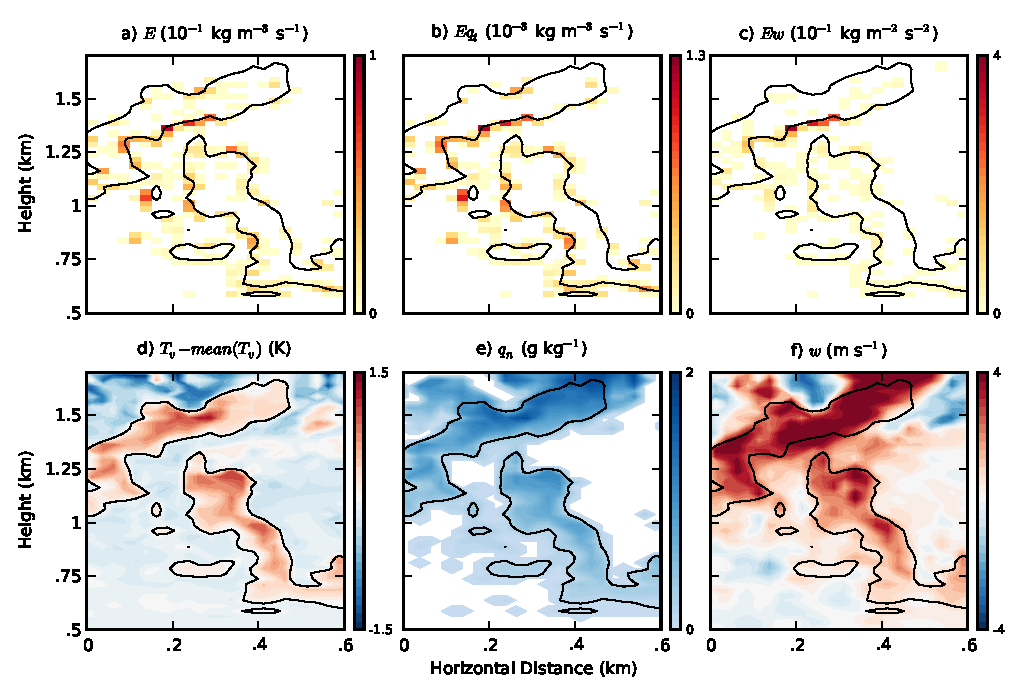
\includegraphics[width=39pc]{./figures/w_entrainment_example}
  \caption{Instantaneous vertical cross-section of cloud core mass entrainment 
  (a), humidity entrainment (b), vertical velocity entrainment (c), buoyancy 
  (d), condensed liquid water (e), and vertical velocity (f) of a single model
  cloud, illustrating the Reynolds correlation between vertical velocity and 
  entrainment.  Black lines indicate the edge of the cloud core in each figure.}
  \label{fig:w_entrainment_example}
\end{figure}


\begin{figure}[t]
  \noindent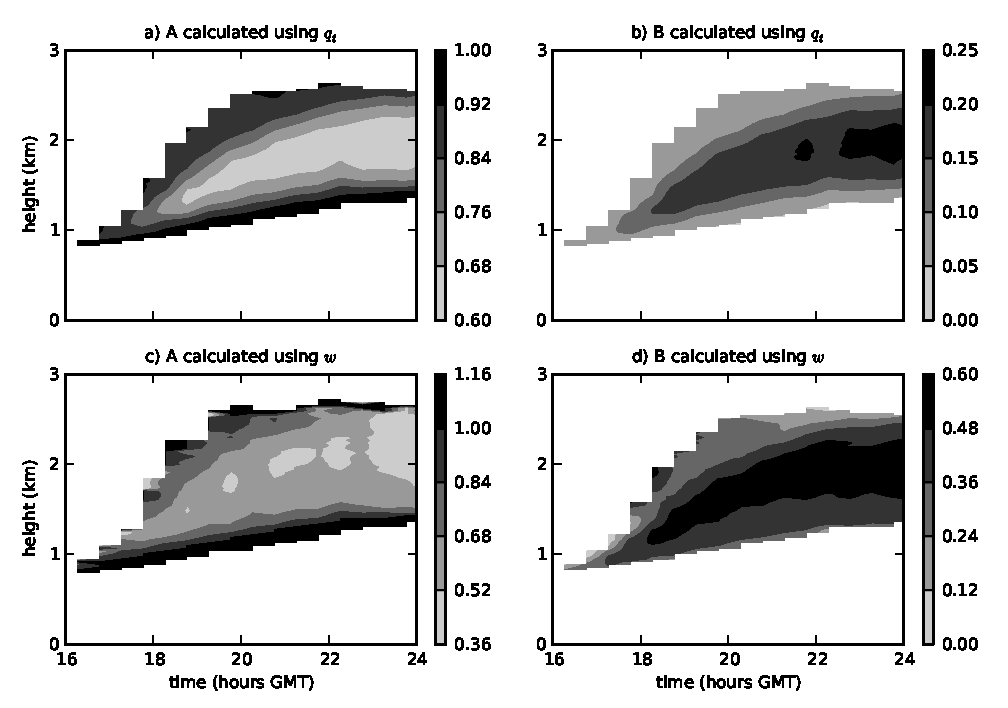
\includegraphics[width=19pc]{./figures/shell_variability}
  \caption{Variation in a) $(q_E - {q_t}_e)/({q_t}_c - {q_t}_e)$ and b)
  $({q_t}_c - q_D)/({q_t}_c - {q_t}_e)$ over the duration of the ARM model run.
  }
  \label{fig:shell_variability}
\end{figure}

\end{document}